\chapter{Access Monitor Plus}

This chapter explains how to use the Access Monitor Plus application.

\section{Homepage}

Figure \ref{fig:amp_homepage}.

\begin{figure}[H]
    \centering
    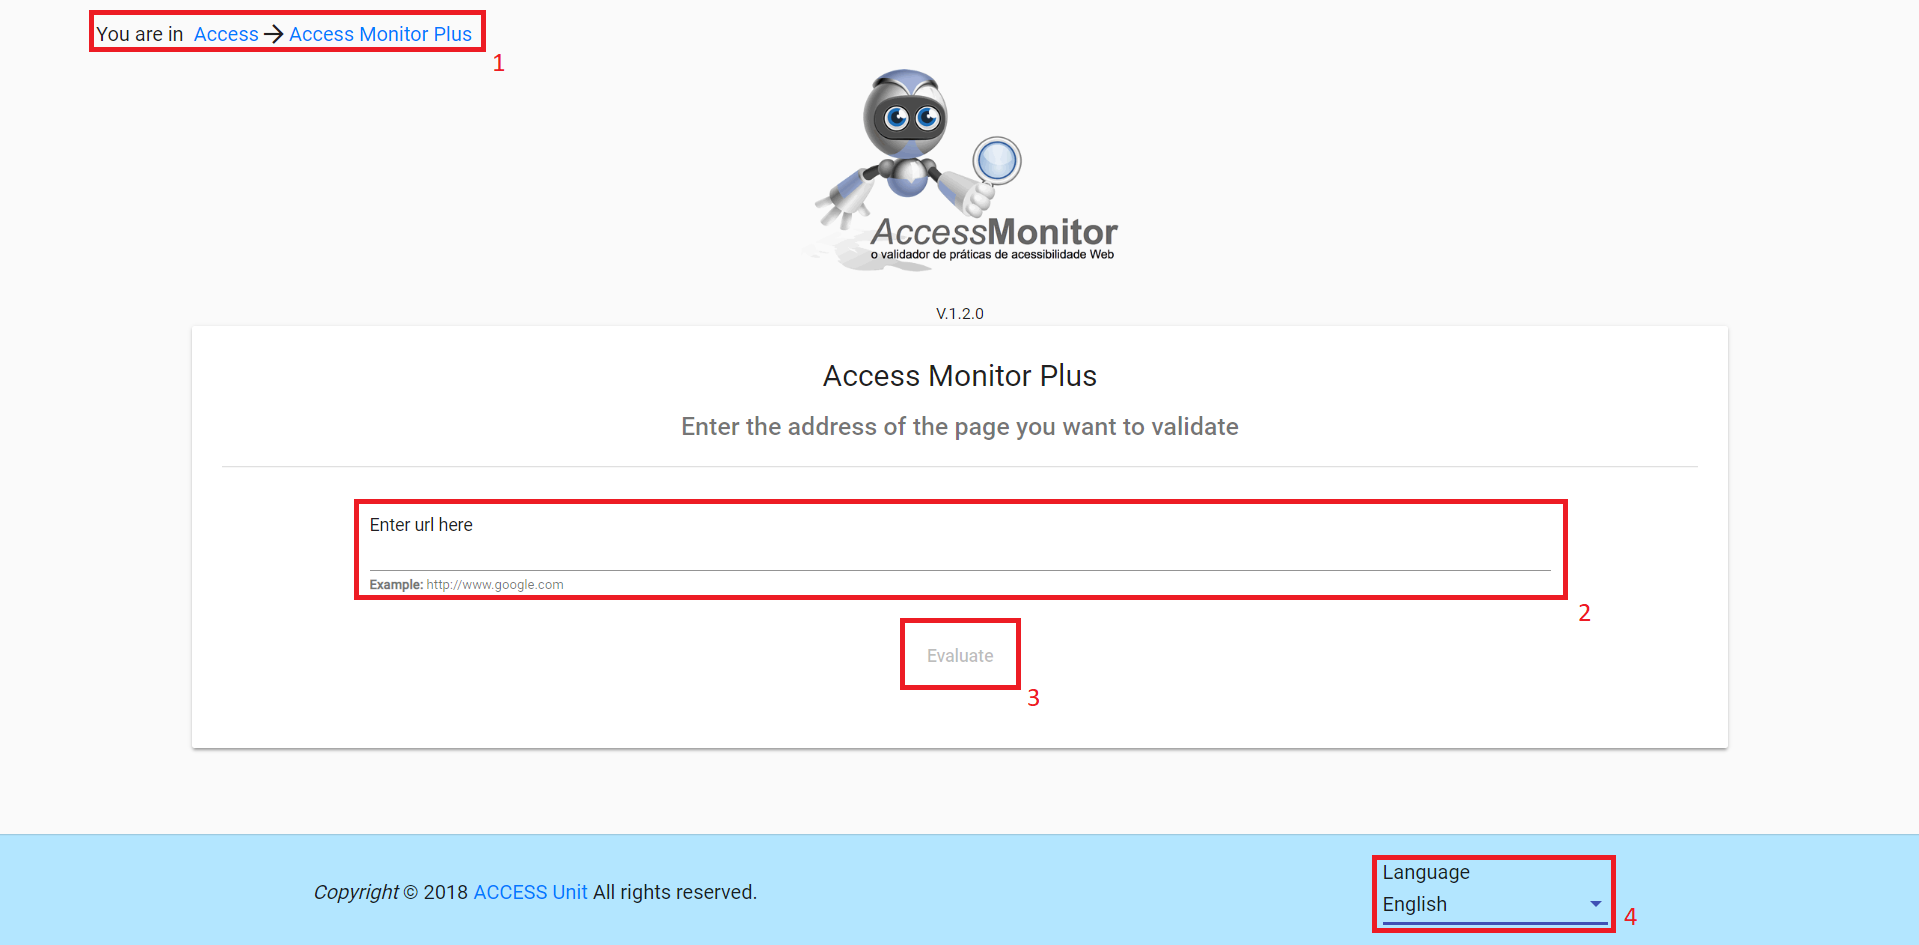
\includegraphics[width=\linewidth]{lib/images/amp/amp_homepage.png}
    \caption{Access Monitor Plus homepage}
    \label{fig:amp_homepage}
\end{figure}

\begin{enumerate}
    \item Breadcrumbs menu
    \item URL form to evaluate webpages
    \item Button to evaluate the inserted URL
    \item Language selection box
\end{enumerate}

\section{Results page}
\label{sec:amp_results_page}

Figures \ref{fig:amp_results_page} - \ref{fig:amp_results_page_2}.

\begin{figure}[H]
    \centering
    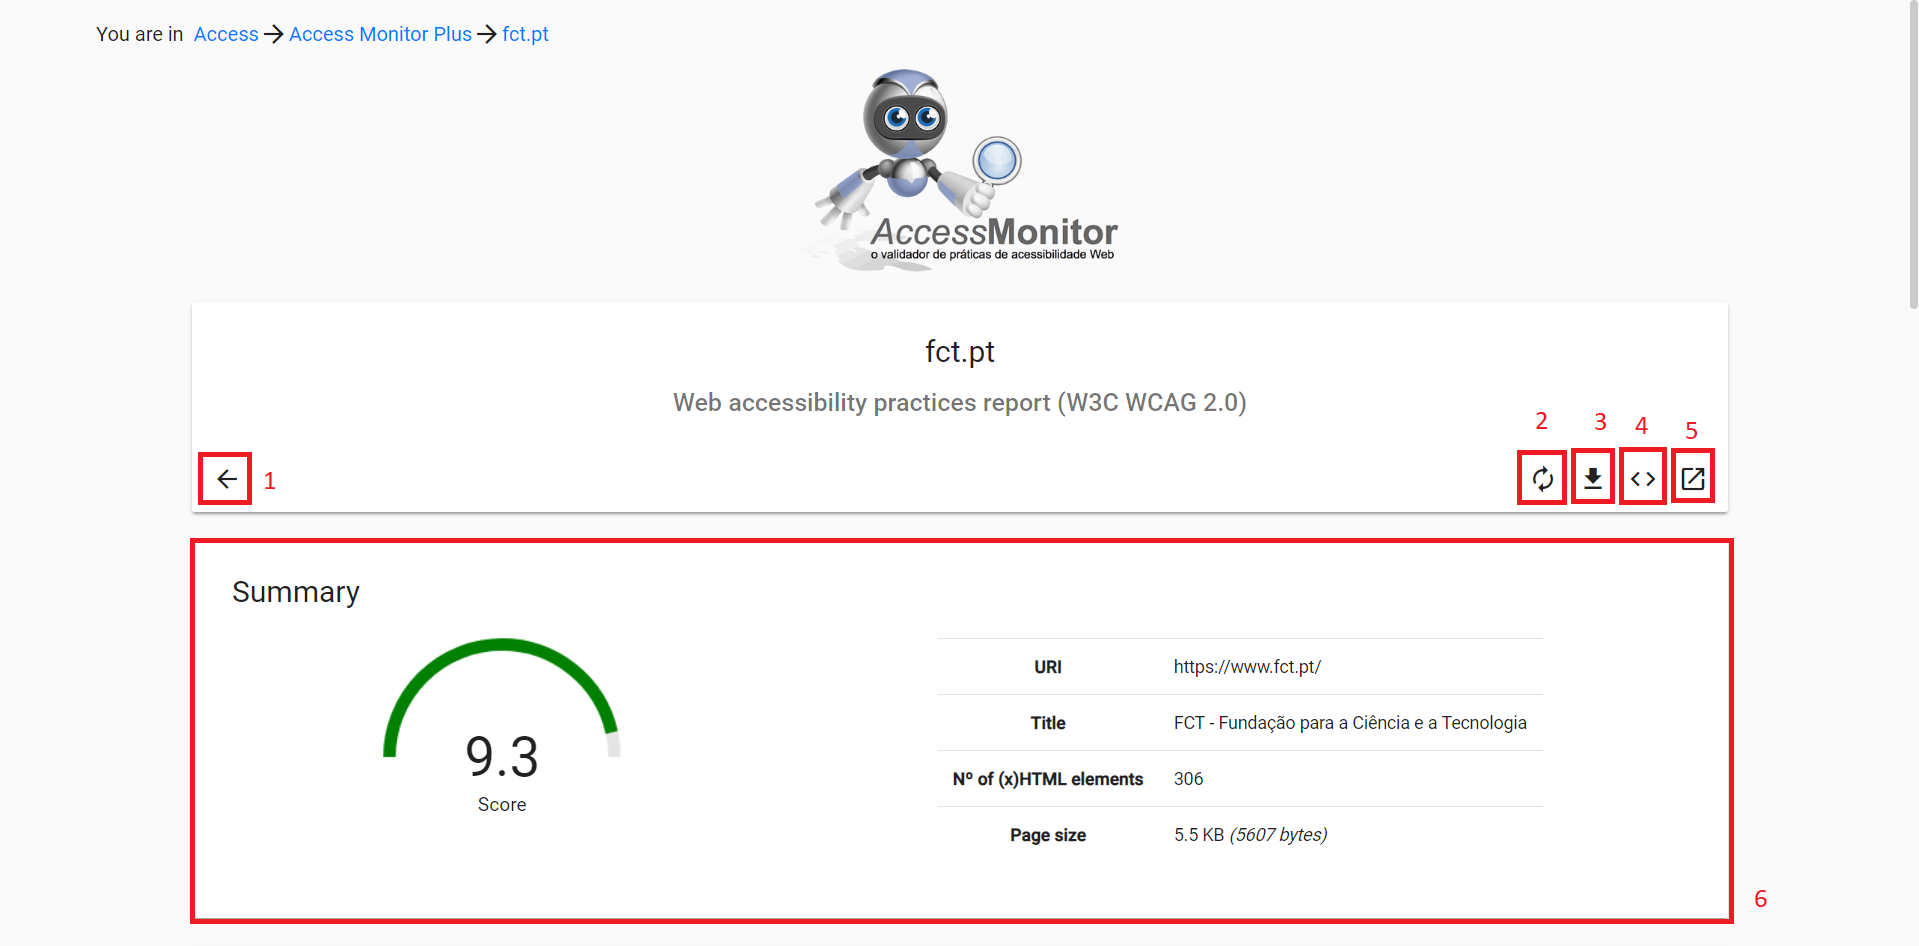
\includegraphics[width=\linewidth]{lib/images/amp/amp_results_page.png}
    \caption{Access Monitor Plus results page}
    \label{fig:amp_results_page}
\end{figure}

\begin{figure}[H]
    \centering
    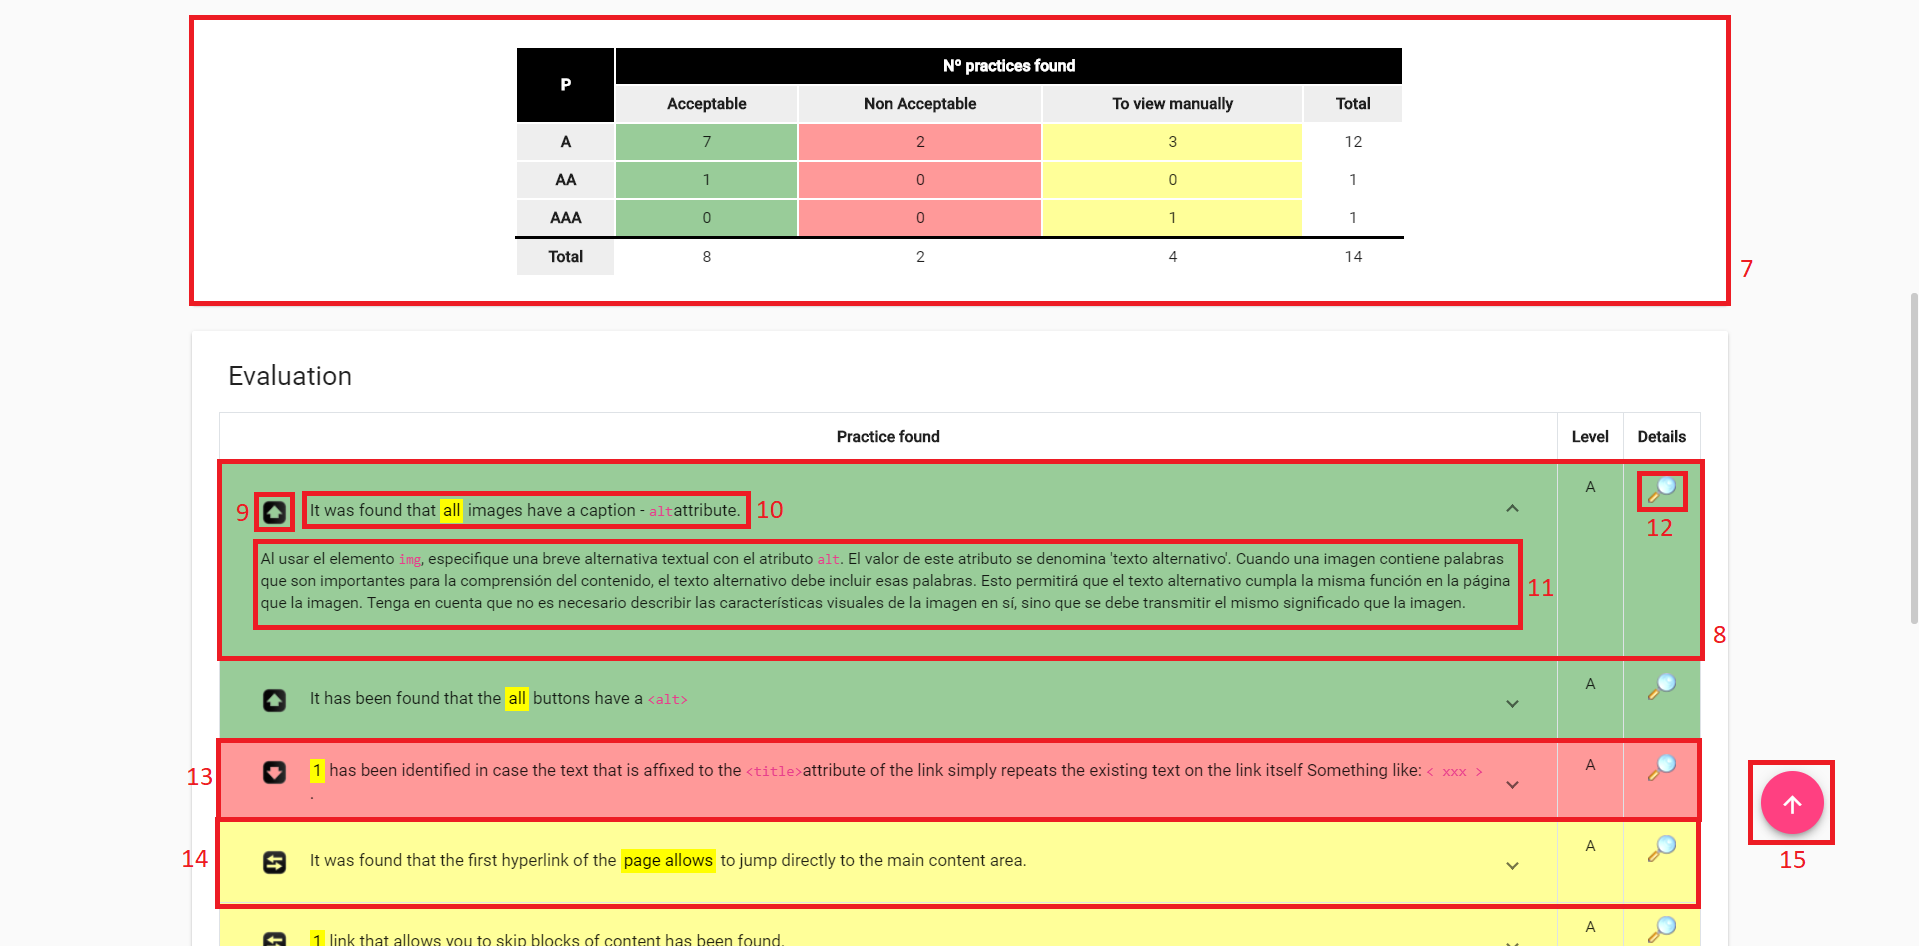
\includegraphics[width=\linewidth]{lib/images/amp/amp_results_page_2.png}
    \caption{Access Monitor Plus results page (cont.)}
    \label{fig:amp_results_page_2}
\end{figure}

\begin{enumerate}
    \item Go back to the previous page (homepage)
    \item Re-evaluates the webapge
    \item Download the evaluation (CSV format)
    \item Go to ``show webpage code'' page
    \item Go to the evaluated webpage
    \item Evaluation metadata summary
    \item Evaluation number of tests categorised
    \item Example of a success practice
    \item Icon that represents the verdict of the practice (success, failed, warning)
    \item Title of the practice
    \item Description of the practice
    \item Goes to the ``element result'' page
    \item Example of a failed practice
    \item Example of a warning practice
    \item ``Go to top'' button
\end{enumerate}

\clearpage

\section{Webpage code page}
\label{sec:amp_webpage_code_page}

Figure \ref{fig:amp_webpage_page}.

\begin{figure}[H]
    \centering
    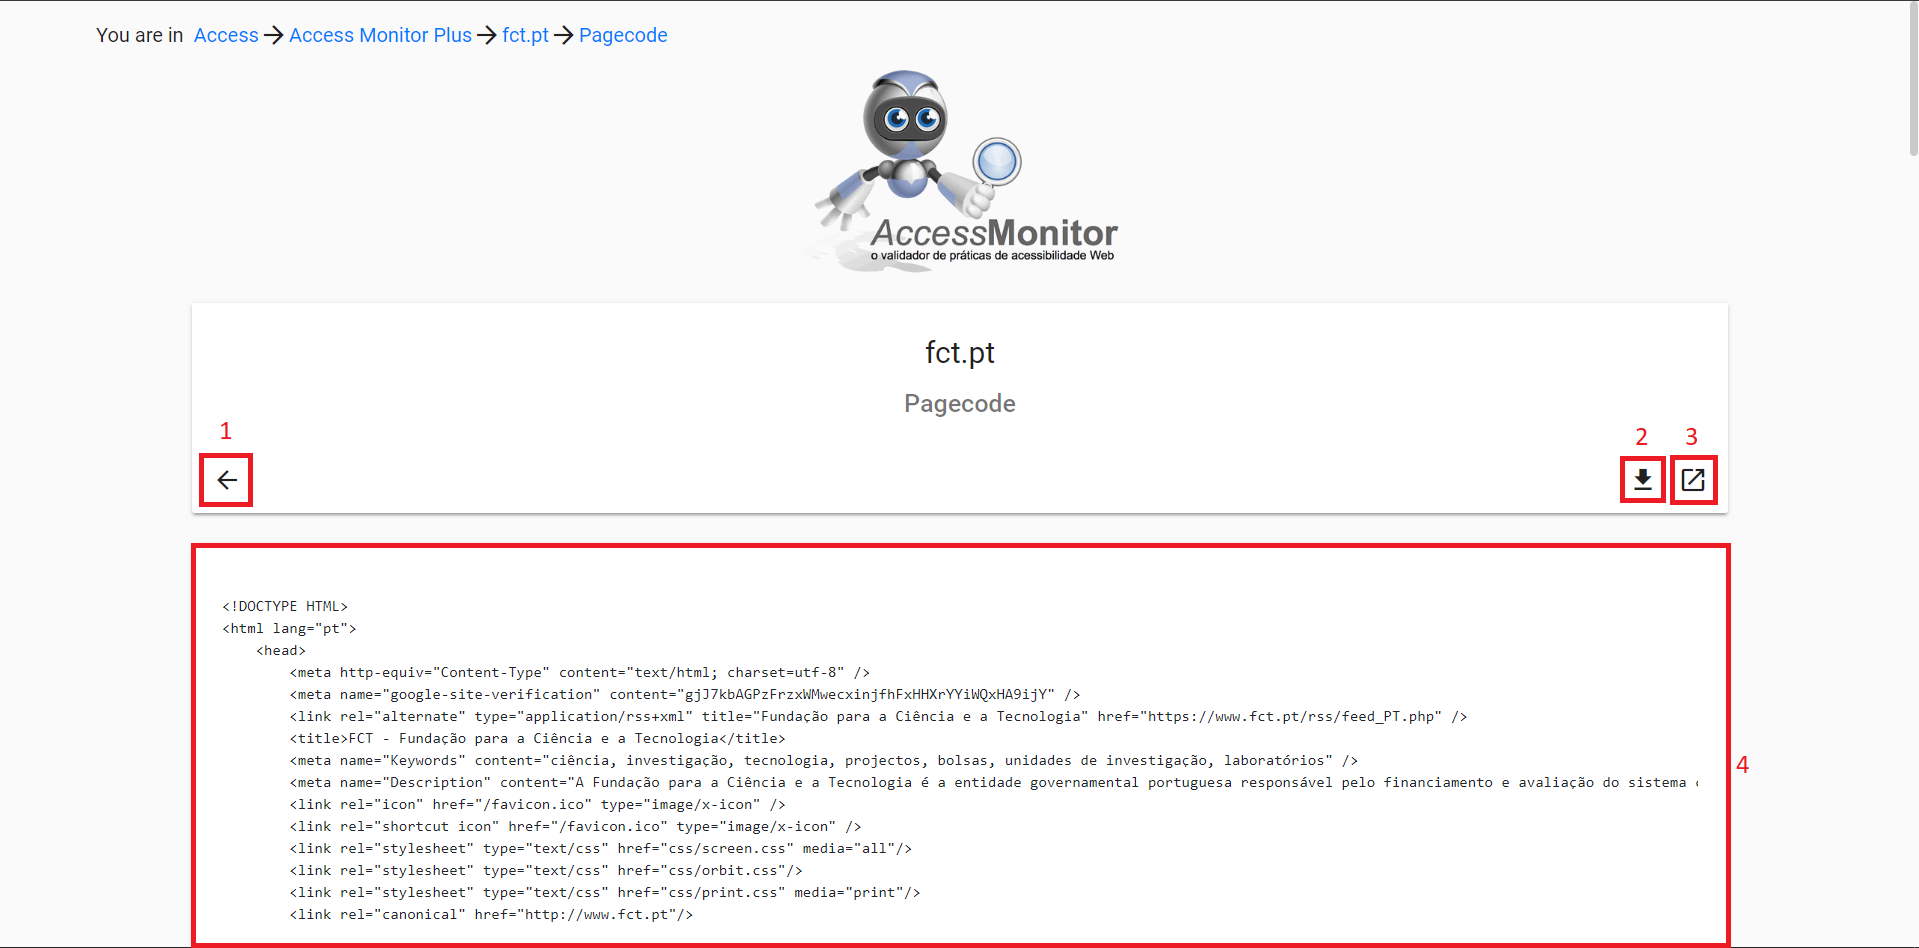
\includegraphics[width=\linewidth]{lib/images/amp/show_webpage_code_page.png}
    \caption{Access Monitor Plus show webpage code page}
    \label{fig:amp_webpage_page}
\end{figure}

\begin{enumerate}
    \item Goes back to the previous page (results page)
    \item Downloads the webapge code
    \item Goes to the evaluated webpage 
    \item Webpage source code (HTML)
\end{enumerate}

\clearpage

\section{Element result page}
\label{sec:amp_element_result_page}

Figures \ref{fig:amp_element_result_page_list} - \ref{fig:amp_element_result_page_page}.

\begin{figure}[H]
    \centering
    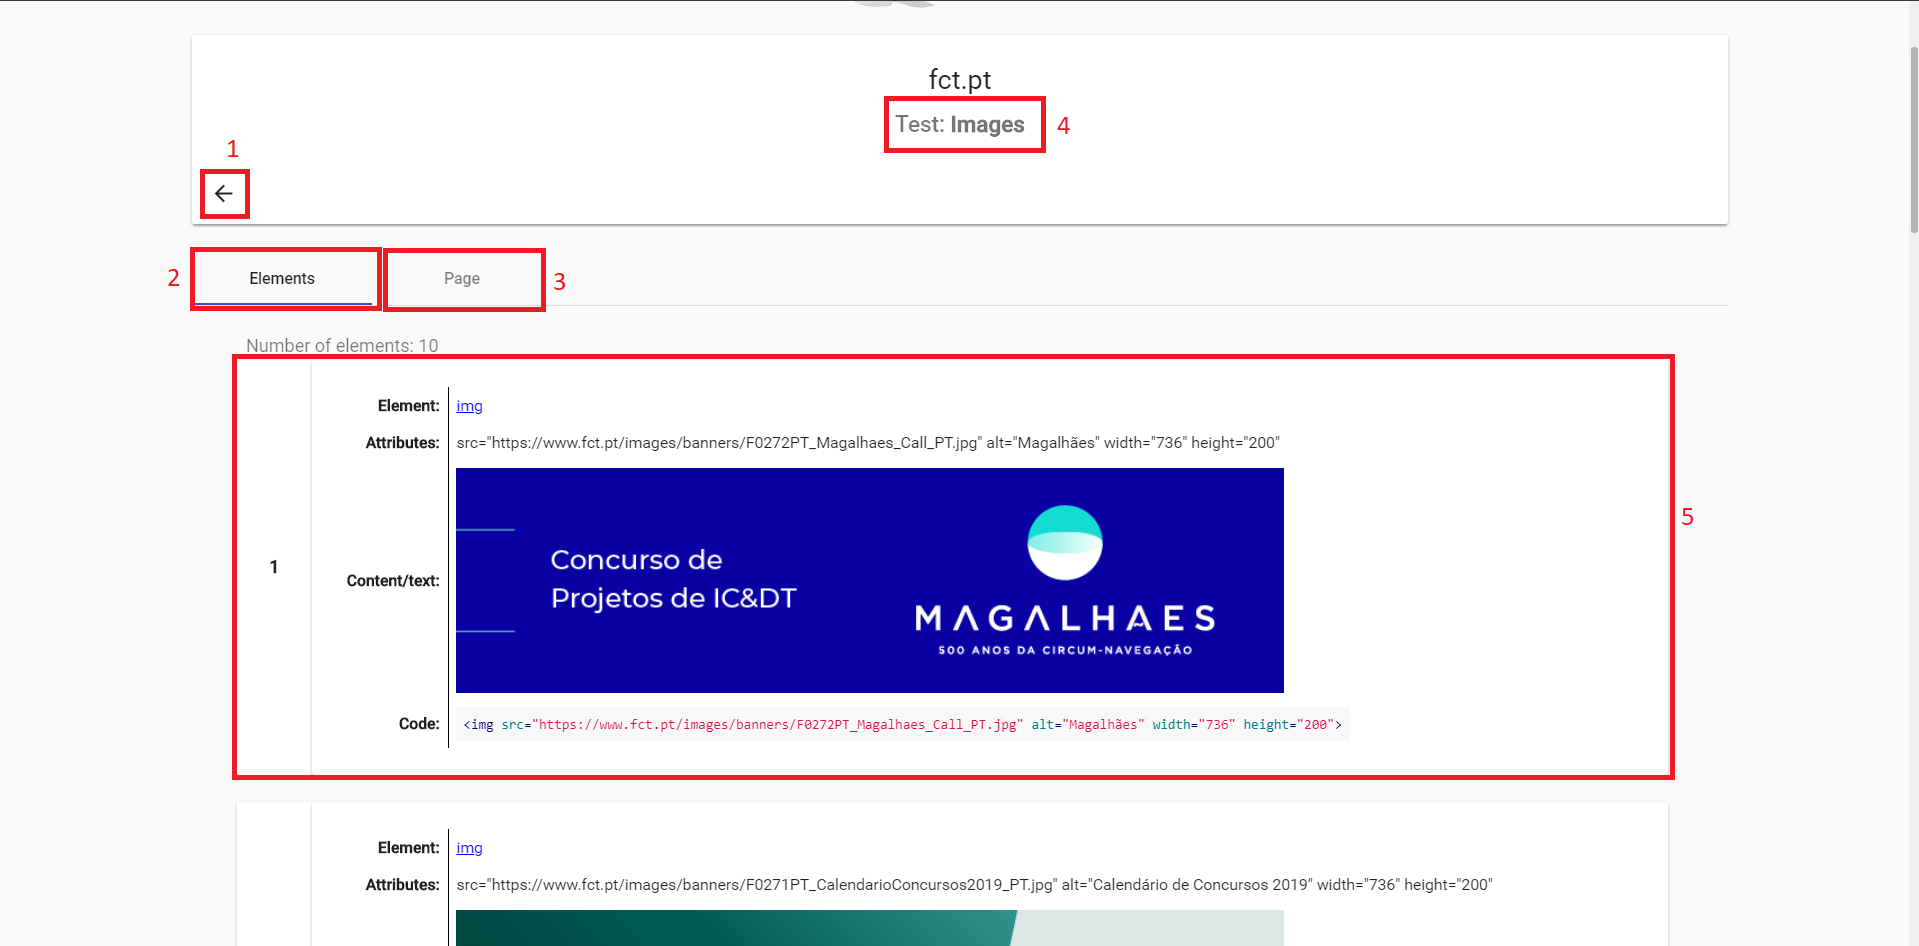
\includegraphics[width=\linewidth]{lib/images/amp/element_result_page_list.png}
    \caption{Access Monitor Plus element result page, list of results}
    \label{fig:amp_element_result_page_list}
\end{figure}

\begin{figure}[H]
    \centering
    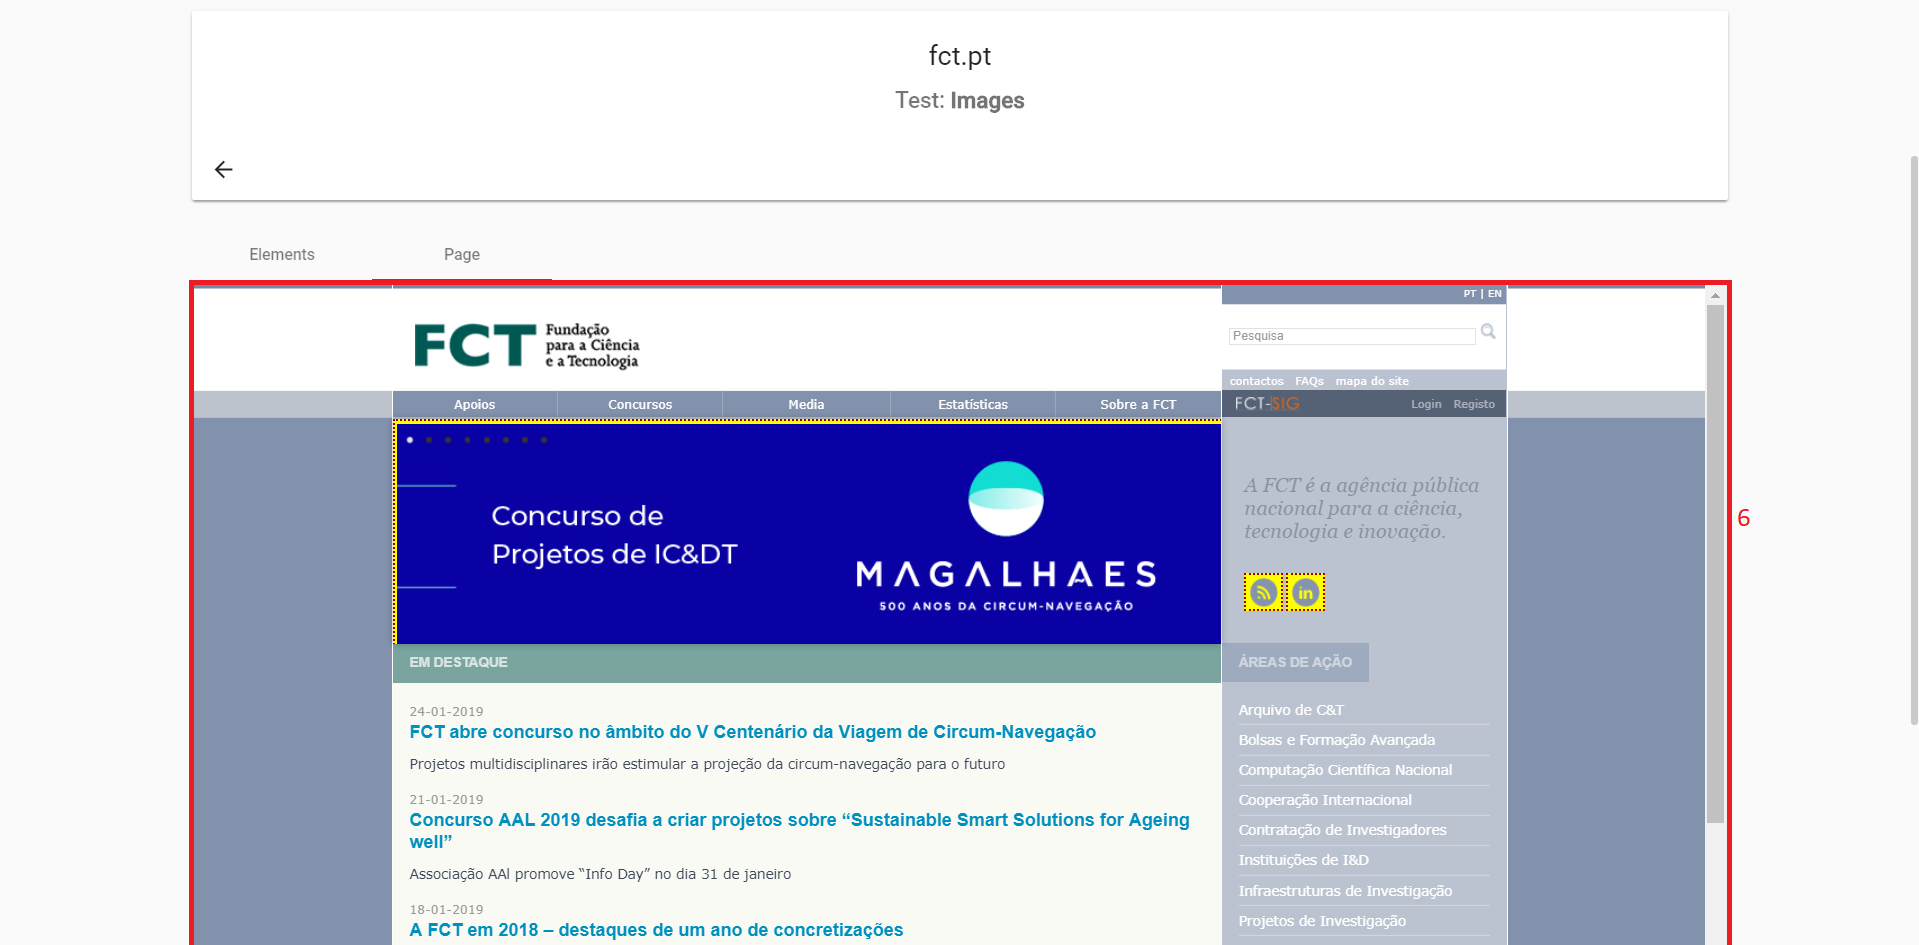
\includegraphics[width=\linewidth]{lib/images/amp/element_result_page_page.png}
    \caption{Access Monitor Plus element result page, results highlighted in page}
    \label{fig:amp_element_result_page_page}
\end{figure}

\begin{enumerate}
    \item Goes back to the previous page (results page)
    \item ``Show list of results'' tab
    \item ``Show elements highlighted in page'' tab
    \item Test evaluated
    \item Example of an element evaluated
    \item Elements highlighted in page
\end{enumerate}